\section{Løsningsalgoritmer}

Der findes indtil flere løsningsalgoritmer til at løse TSP. Det viser sig dog imidlertid, at der ikke er nogen let måde, at løse problemet på. Som tidligere nævnt, er det nødvendigt at ty til approksimationsalgoritmer for at have en chance for at finde en nogenlunde brugbar løsning.

Den mest umiddelbart løsningsalgoritme til at finde en korteste Hamiltonkreds rundt i en graf, finder samtlige mulige Hamiltonkredse i grafen. Til hver af disse kredse beregnes den samlede vægt, og til sidst sammenlignes alle disse samlede vægte, for at finde den Hamiltonkreds, som har den mindste samlede vægt. Denne algoritme er i pseudokode beskrevet i Algoritme \ref{brute_force}.

\begin{algorithm}
\caption{Brute-force algoritmen}
\label{brute_force}
\textbf{procedure} Find korteste Hamiltonkreds i grafen $G$ med $\alpha$ Hamiltonkredse.

Bestem alle Hamiltonkredse, $H_k$, i $G$, og lad $H_{ki}$ betegne den $i$'te Hamiltonkreds. \\
\textbf{for} $i:=1$ til $\alpha$ \\
$\-$ $\-$ $\-$ $\-$ $\-$ $\-$
Bestem $d(H_{ki})$ \\
$min := H_{k1}$ \\
\textbf{for} $i:=2$ til $\alpha$ \\
$\-$ $\-$ $\-$ $\-$ $\-$ $\-$
\textbf{hvis} $min > H_{ki}$ \textbf{så} $min := H_{ki}$ \\
\textbf{returnér} $min$ $\lbrace$ $min$ er den korteste Hamiltonkreds i $G$ $\rbrace$
\end{algorithm}

Denne algoritme vil altid finde den korteste Hamiltonkreds i en komplet graf $G$, men kræver meget processorkraft at gennemføre, selv for grafer med relativt få knuder \citep{dmat}.

\begin{thm}
Den værst mulige tidskompleksitet af Brute-force Algoritmen er $O(n!)$.
\end{thm}

\begin{proof}
Lad $G$ være en komplet graf med $n$ knuder og $n \geq 3$. I denne graf er der så $(n-1)!$ forskellige Hamiltonkredse, idet de $n-1$ punkter kan arrangeres på $(n-1)!$ forskellige måder. Derfor har algoritmen allerede her en værst mulig tidskompleksitet på $O(n!)$ idet $(n-1)!$ er $O(n!)$. 

Herfter foretager algoritmen en lineær søgning, som jf. Eksempel \ref{eks_lin_soeg} har en værst mulig tidskompleksitet på $\Theta(n)$, og spiller derfor ingen rolle i algoritmens samlede kompleksitet.
\end{proof}

Brute-force algoritmen har således en kompleksitet, der er voldsom stor selv ved relativt få knuder i $G$.

\begin{exmp}
I den komplet graf, $G$, med $20$ knuder, har brute-force algoritmen en værst mulig tidskompleksitet på $$20! = 2432902008176640000,$$ hvorfor algoritmen tydeligvis allerede ved $20$ knuder er håbløs.
\end{exmp}

Derfor er approksimationsalgoritmer nødvendige, for at løse problemet. Som tidligere beskrevet, vil disse algoritmer \textit{ikke} finde den optimale løsning, men en løsning, som ligger indenfor en vis konstant grænse. I denne rapport vil Dobbelttræ-algoritmen anvendes til at løse TSP. 

\subsection{Dobbelttræ-algoritmen}
Dobbelttræ-algoritmen forudsætter, at grafen, som Hamiltonkredsen skal findes i, er komplet metrisk. For sådanne grafer kan der imidlertid foretages en \textit{genvej}, som defineres i Definition \ref{def_genvej}.

\begin{defn}
Lad $G$ være en komplet, metrisk graf med $n$ knuder og $n \geq 3$. I $G$ findes en vej, $P = v_0, v_1,...,v_{i-1}, v_i, v_{i+1},...,x_{n-1},x_n$ hvor $1 \leq i \leq n-1$. \\
I $P$ findes så to kanter $e_i = \lbrace x_{i-1}, x_i \rbrace$ og $e_{i+1} = \lbrace x_i, x_i+1 \rbrace$, så $e_i \cap e_{i+1} = x_i$.
Der findes så en trekant $\Delta_i = \lbrace e_i, e_{i+1}, e_s \rbrace$ i $G$, hvor $e_s = \lbrace x_{i-1}, x_{i+1} \rbrace$.
Da kan der dannes en genvej i $P$ via $e_s$ således en ny vej, $P'=v_0, v_1,...,x_{i-1},x_{i+1},...,x_{n+1},x_n$, dannes.
Idet $G$ er metrisk opfylder den trekantsuligheden, så $d(e_s) \leq d(e_i) + d(e_{i+1})$ og dermed er $d(P') \leq d(P)$.
\label{def_genvej}
\end{defn}

Dobbelttræ-algoritmen begynder med, i en komplet, metrisk graf $G$, at finde et minimalt udspændende træ, $T$, som kan findes ved hjælp af Prims Algoritme. Når $T$ er fundet, fordobles alle kanter i $T$, som så danner en multigraf $D$. Graden af alle knuder i denne grad må være lige, hvorfor der må eksistere en Eulerkreds i $D$, jf. Sætning \ref{Eulerkreds_multigraf}. Eulerkredsen dannes ved Algoritme \ref{algoritme_euler}.  I denne Eulerkreds skydes der genvej, for at opnå en Hamiltonkreds, $H$. Denne algoritme er sammenfattet i Algoritme \ref{dt_algo}. 

\newpage
\begin{algorithm}[h]
\caption{Dobbelttræ-algoritme}
\label{dt_algo}
\textbf{procedure} En metrisk komplet graf, $G$ \\
Find minimalt udspændende træ, $T$, i $G$ $\lbrace$ Prims Algoritme $\rbrace$. \\
$D := T$ \\
\textbf{for} kant \textbf{i} $D$ \\
$\-$ $\-$ $\-$ $\-$ $\-$ $\-$
dublér kant \\
Find Eulerkreds, $E$, i $D$ \\
Skyd genvej i $E$ for at opnå Hamiltonkredsen, $H$ \\
\textbf{returnér} $H$ $\lbrace$ $H$ er Hamiltonkreds i $G$ $\rbrace$
\end{algorithm}

\begin{exmp}
Som eksempel på Dobbelttræs-Algoritmens fremgangsmåde, ses på en komplet, metrisk graf med $5$ knuder.
På Figur \ref{dtex1} ses grafen, som der nu skal findes en Hamiltonkreds i. Algoritmen finder så er minimalt udspændende træ ved Prims algoritme som i Figur \ref{dtex2}. Herefter ses bort fra de resterende kanter, som ikke er en del af træet, og samtlige kanter i det minimalt udspændende træ fordobles, som det er gjort i Figur \ref{dtex3}. Slutteligt skydes der genvej, som på Figur \ref{dtex4} ses som den røde kant, som indsættes til fordel for de stiplede kanter. Dermed er der fundet en Hamiltonkreds.

\begin{figure}[h]
\centering
	\begin{subfigure}{0.5\textwidth}
		\centering
			\scalebox{0.7}{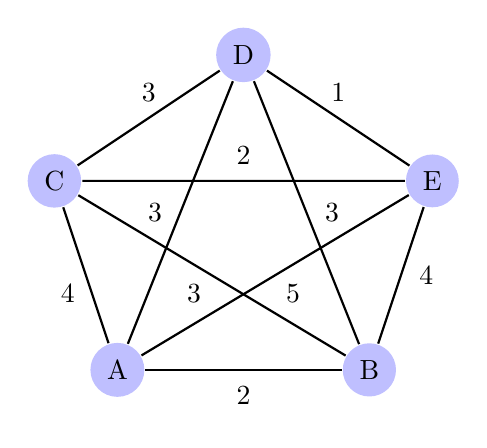
\begin{tikzpicture}
[thick,scale=.8,auto=left,every node/.style={circle,fill=blue!25}]
  \node (na) at (2,0) {A};
  \node (nb) at (6,0) {B};
  \node (nc) at (1,3) {C};
  \node (nd) at (4,5) {D};
  \node (ne) at (7,3) {E};
  \path[-,draw,thick,black]
  	(na) edge node[draw=none,fill=none,below] {$2$} (nb)
  	(nb) edge node[draw=none,fill=none,right] {$4$} (ne)
  	(ne) edge node[draw=none,fill=none,above] {$1$} (nd)
  	(nd) edge node[draw=none,fill=none,above] {$3$} (nc)
  	(nc) edge node[draw=none,fill=none,below left] {$3$} (nb)
  	(na) edge node[draw=none,fill=none] {$4$} (nc)
  	(na) edge node[draw=none,fill=none,below right] {$5$} (ne)
  	(na) edge node[draw=none,fill=none,left] {$3$} (nd)
  	(nd) edge node[draw=none,fill=none,right] {$3$} (nb)
  	(nc) edge node[draw=none,fill=none] {$2$} (ne);
\end{tikzpicture}

  %\path[-,draw,black]
  	%(n3) edge node[draw=none,fill=none] {$e$} (n7);
  %\path[-,draw,very thick,blue,bend right]
  	%(n6) edge node[draw=none,fill=none,color=black] {$e'$} (n7);
  	
  	
 	%\node (n6) at (2,0) {A};
  %\node (n4) at (6,0) {B};
  %\node (n5) at (0,4) {C};
  %\node (n1) at (4,6) {D};
  %\node (n2) at (8,4) {E};
  %\foreach \from/\to in {n6/n5,n4/n2}
    %\draw (\from) -- (\to);}
		\label{dtex1}
		\caption{Komplet vægtet metrisk graf med $5$ knuder.}
	\end{subfigure}%
	\begin{subfigure}{0.5\textwidth}
		\centering
			\scalebox{0.7}{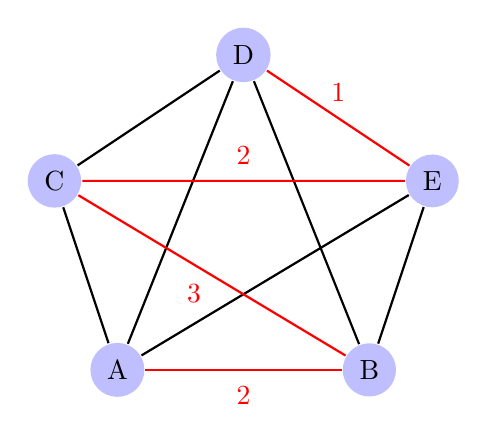
\begin{tikzpicture}
[thick,scale=.8,auto=left,every node/.style={circle,fill=blue!25}]
  \node (na) at (2,0) {A};
  \node (nb) at (6,0) {B};
  \node (nc) at (1,3) {C};
  \node (nd) at (4,5) {D};
  \node (ne) at (7,3) {E};
  \path[-,draw,thick,black]
  	(ne) edge (nb)
  	(nd) edge (nc)
  	(na) edge (nc)
  	(na) edge (ne)
  	(na) edge (nd)
  	(nd) edge (nb);
  	
  \path[-,draw,thick,red]
  	(na) edge node[draw=none,fill=none,below] {$2$} (nb)
  	(nc) edge node[draw=none,fill=none,below left] {$3$} (nb)
  	(nc) edge node[draw=none,fill=none] {$2$} (ne)
  	(ne) edge node[draw=none,fill=none,above] {$1$} (nd);
\end{tikzpicture}}
		\label{dtex2}
		\caption{Minimalt undspændende træ findes i grafen.}
	\end{subfigure}
	\newline
	\begin{subfigure}{0.5\textwidth}
		\centering		
			\scalebox{0.7}{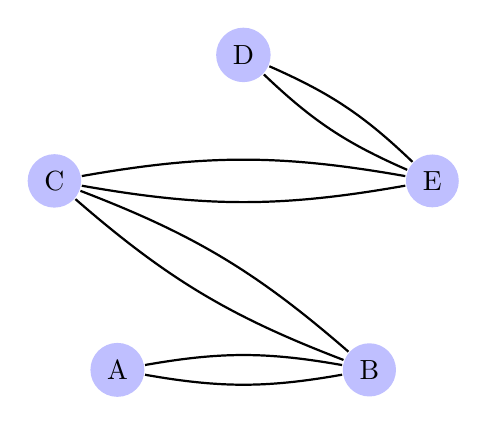
\begin{tikzpicture}
[thick,scale=.8,auto=left,every node/.style={circle,fill=blue!25}]
  \node (na) at (2,0) {A};
  \node (nb) at (6,0) {B};
  \node (nc) at (1,3) {C};
  \node (nd) at (4,5) {D};
  \node (ne) at (7,3) {E};

  \path[-,draw,thick,black,bend right=10]
  	(na) edge (nb)
  	(nc) edge (nb)
  	(nc) edge (ne)
  	(ne) edge (nd);
  
  \path[-,draw,thick,black,bend left=10]
  	(na) edge (nb)
  	(nc) edge (nb)
  	(nc) edge (ne)
  	(ne) edge (nd);
\end{tikzpicture}}
		\label{dtex3}
		\caption{Alle kanter i træet fordobles.}
	\end{subfigure}%
	\begin{subfigure}{0.5\textwidth}
		\centering
			\scalebox{0.7}{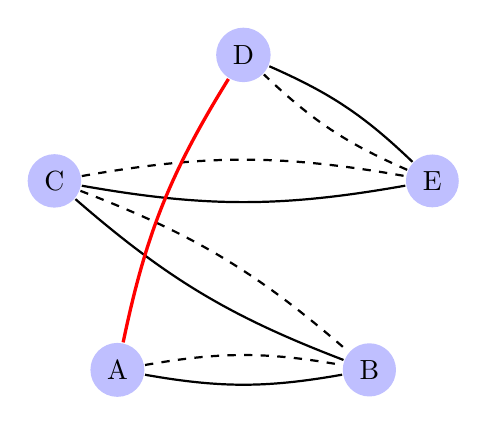
\begin{tikzpicture}
[thick,scale=.8,auto=left,every node/.style={circle,fill=blue!25}]
  \node (na) at (2,0) {A};
  \node (nb) at (6,0) {B};
  \node (nc) at (1,3) {C};
  \node (nd) at (4,5) {D};
  \node (ne) at (7,3) {E};

  \path[-,draw,thick,black,bend right=10]
  	(na) edge (nb)
  	(nc) edge (nb)
  	(nc) edge (ne)
  	(ne) edge (nd);
  
  \path[dashed,draw,thick,black,bend left=10]
  	(na) edge (nb)
  	(nc) edge (nb)
  	(nc) edge (ne)
  	(ne) edge (nd);
  	
  \path[-,draw,very thick,red,bend right=10]
  	(nd) edge (na);
  	
\end{tikzpicture}}
		\label{dtex4}
		\caption{Der skydes genvej i Eulerkredsen\\ for at
		danne en Hamiltonkreds.}
	\end{subfigure}
\end{figure}
\end{exmp}

Dobbelttræ-algoritmen approksimerer den Hamiltonkreds, som er af lavest mulig vægt.

\begin{thm}
Dobbelttræ-algoritmen er en 2-approksimationsalgoritme.
\end{thm}

\begin{proof}
Lad $H'$ være Hamiltonkredsen af lavest muligt vægt i grafen $G$ og $H$ være den Hamiltonkreds, som Dobbelttræ-algoritmen finder ved genvej i Eulerkredsen $E$. Da må der gælde, at $$d(H)\leq d(E).$$ 
Idet Eulerkredsen, $E$, er dannet ved at dublere alle kanter i det minimalt udspændende træ, $T$, må der gælde, at $$d(E) = 2d(T).$$
Idet enhver Hamiltonkreds ved fjernelse af en kant danner et udspændende træ, må der i $H'$'s tilfælde gælde, at $d(T) \leq d(H')$. Heraf følger det, at $$2d(T) \leq 2d(H').$$
Derfor må der gælde, at $$d(H) \leq 2d(H'),$$ hvorfor Dobbelttræ-algoritmens fundne Hamiltonkreds, $H$, ikke har en vægt større end $2d(H')$. 
\end{proof}

\subsection{Kompleksitet af Dobbelttræ-algoritmen}
Dobbelttræ-aalgoritmen er en approksimationsalgoritme, som det er bevist ovenfor. Derfor må det formodes, at den har en lavere kompleksitet end Brute-force Algoritmen havde.

\begin{thm}
Dobbelttræ-algoritmen har en værst mulig tidskomplesitet på $O(n^3)$.
\end{thm}

\begin{proof}
Dobbelttræ-algoritmen gennemkører først Prims Algoritme, som er $O(n^3)$, jf. Sætning \ref{prim_kompl}. 
Derefter fordobler algoritmen samtlige sider i træet, som Prims Algoritme har dannet. Denne tilfører kompleksiteten $O(n)$.
Så gennemkører Dobbelttræ-algoritmen algoritmen for dannelsen af en Eulerkreds, som har lineær værst mulig tidskompleksitet, altså også $O(n)$.
Slutteligt vil Dobbelttræ-algoritmen skyde genvej ved at gennemgå den dannede Hamiltonkreds, hvilket også har lineær værst mulig tidskompleksitet. 
Derfor må den værst mulige tidskompleksitet af Dobbelttræ-algoritmen være $O(n^3)$.
\end{proof}

Dobbelttræ-algoritmen viser sig altså at være af polynomiel værst mulig tidskompleksitet, hvorfor denne noget hurtigere vil finde en kort Hamiltonkreds i grafen. Dog er det på kompromis at, at det ikke nødvendigvis er den korteste Hamiltonkreds i $G$.

\begin{exmp}
I den komplette graf, $G$, med $20$ knuder, har Dobbelttræ-algoritmen en værst mulig tidskompleksitet på $$20^3 = 8000,$$ og er derfor markant hurtigere end Brute-force Algoritmen.
\end{exmp}




